\documentclass[12pt]{article}
\usepackage[utf8]{inputenc}
\usepackage{amsmath,amsfonts}
\usepackage{hyperref}
\usepackage{tikz}
\usepackage{pgfplots}
\usepackage{xcolor}
\usepackage[left=2cm,right=2cm,top=3cm,bottom=3cm,footskip=0cm,foot=1cm,marginparsep=0cm,marginparwidth=1cm,headsep=0.5cm,headheight=1cm]{geometry}

\definecolor{myblue}{rgb}{0.00,0.39,0.67}
\definecolor{myred}{rgb}{0.86,0.08,0.14}
\definecolor{mygreen}{rgb}{0.07,0.52,0.07}
\definecolor{myorange}{rgb}{0.99,0.32,0.08}
\definecolor{mygray}{rgb}{0.5,0.5,0.5}


\def\Ef{\eta}
\def\happy{\mathcal{H}}
\def\gym{\mathcal{G}}
\def\bonus{\mathcal{B}}

\def\Sc{S_\text{c}}
\def\Si{S_\text{i}}
\def\Sf{S_\text{f}}
\def\Ec{E_\text{c}}

\title{Battle stats formula}
\author{Kivou [2000607]}

\begin{document}
\maketitle
\par {\it Starting from a formula that gives the battle stats gains for a certain amount of energy, we derive here  a formula that gives the battle stats as a function of energy and, in turns, the energy needed to reach a certain battle stats level from a given one.}

\section{Gym gain formula}
\href{https://www.torn.com/forums.php?p=threads&f=61&t=16003284&b=0&a=0&start=0&to=17684755}{Vladar [1996140]} gives a formula defining the battle stats gains as a function of the current stat, the energy spent on train and other parameters.

\par In this formula and for the rest we will need:
\begin{itemize}
    \item 2 variables and their increments
    \begin{itemize}
        \item Energy $E$ and $dE$
        \item Battle stats $S$ and $dS$
    \end{itemize}
    \item 6 known coefficients
        \begin{itemize}
            \item $a = 0.0000003480061091$
            \item $b = 250$
            \item $c = 0.000003091619094$
            \item $d = 0.0000682775184551527$
            \item $e = -0.0301431777$
            \item $\Sc = 50000000$ (known as the battle stats cap)
        \end{itemize}
    \item 3 states variables
    \begin{itemize}
        \item Happy level $\happy$
        \item Gym coefficient $\gym$
        \item Gym gain bonus $\bonus$
    \end{itemize}
\end{itemize}

The Valdar formula eq.\eqref{eq:valdar} gives the stats gains $dS$ as a function of the current stats $S$ and the energy spent $dE$. It is usually written:
\begin{equation}
    dS = \left[ (a\ln(\happy+b)+c) \bar{S} + d(\happy+b) + e \right](1+\bonus)\gym dE
    \label{eq:valdar}
\end{equation}
with $\bar{S} = \min(\Sc, S)$

\par By introducing 2 new parameters $\alpha$ and $\beta$ that depend only on the 5 coefficients $a, b, c, d, e$ and the state variables $\happy, \bonus, \gym$, eq.\eqref{eq:valdar} can be written as follow:
\begin{equation}
    \frac{dS}{dE} = \alpha \bar{S} + \beta \quad \Leftrightarrow \quad \frac{dS}{dE} - \alpha \bar{S} = \beta
    \label{eq:valdar-diff}
\end{equation}
with
\begin{equation}
    \left\{\begin{aligned}
        \alpha &= (a\ln(\happy+b)+c)(1+\bonus)\gym\\
        \beta &= (d(\happy+b) +e)(1+\bonus)\gym
    \end{aligned}\right.
\end{equation}
From now on we assume that $\alpha > 0$ and $\beta > 0$.

\section{Battle stats formula: $S(E)$}
\par {\color{myred}\bf Assumption: $\happy$, $\gym$ and $\bonus$ remain constant (which is not realistic for a long term prediction at early stages).}

\par From eq.\eqref{eq:valdar-diff} it can clearly be seen that $S(E)$ is driven by a simple ODE. Because of the piece wise definition of the equation the two cases $S<\Sc$ (before cap) and $S>\Sc$ (after cap) have to be treated separatly.

\subsection{Before cap}
With $S<\Sc$ eq.\eqref{eq:valdar-diff} can be written:
\begin{equation}
    \frac{dS}{dE} -\alpha S = \beta
\end{equation}
Which leads to the solution:
\begin{equation}
    \forall k \in \mathbb{R},\quad S(E) = ke^{\alpha E} - \frac{\beta}{\alpha}
    \label{eq:bs-bc-diff-k}
\end{equation}
With the initial condition $S(0)=0$ we have
\begin{equation}
    S(E) = \frac{\beta}{\alpha}\left(e^{\alpha E} - 1\right)
    \label{eq:bs-bc-diff}
\end{equation}

It can be interesting to compute $E=\Ec$ such that $S(\Ec)=\Sc$ which can be done by inverting eq.\eqref{eq:bs-bc-diff}. It gives:
\begin{equation}
    \Ec = \frac{1}{\alpha}\ln\left(\frac{\alpha \Sc}{\beta} +1 \right)
\end{equation}

\subsection{After cap}
With $S<\Sc$ eq.\eqref{eq:valdar-diff} can be written:
\begin{equation}
    \frac{dS}{dE}  = \alpha \Sc + \beta
\end{equation}
which directly yields
\begin{equation}
    \forall k \in \mathbb{R},\quad S(E)  = (\alpha \Sc + \beta) E + k
\end{equation}
With the condition $S(\Ec)=\Sc$ we have:
\begin{equation}
    \begin{aligned}
        S & = (\alpha \Sc + \beta)E + \Sc - (\alpha \Sc + \beta) \Ec \\
          & = (\alpha \Sc + \beta) (E - \Ec) + \Sc
    \end{aligned}
\end{equation}
\begin{figure}[!h]
    \centering
    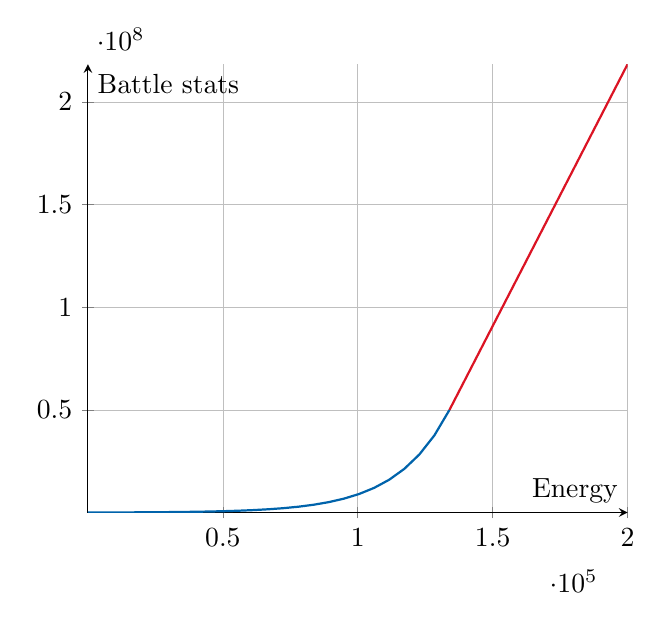
\begin{tikzpicture}
        \begin{axis}[
            % xmin=0,xmax=5000000,
            % ymin=0,ymax=100000000,
            grid=both,
            grid style={line width=.1pt, draw=gray!10},
            major grid style={line width=.2pt,draw=gray!50},
            axis lines=middle,
            % minor tick num=4,
            % ticks=none,
            ylabel=Battle stats,
            xlabel=Energy
        ]

           % \def\alpha{0.0000052543};
           % \def\beta{0.0039955815};
           % \def\ec{2111332.2434403603};
           % \def\sc{50000000)};
           % \addplot[myblue, domain=0:\ec, thick]{ \beta * (exp(\alpha * x) - 1) / \alpha };
           % \addplot[myred, domain=\ec:2500000, thick]{ (\alpha * \sc + \beta) * (x - \ec) + \sc };
           \def\alpha{0.0000509798};
           \def\beta{2.7561943022};
           \def\ec{133988.1087149439};
           \def\sc{50000000)};
           \addplot[myblue, domain=0:\ec, thick]{ \beta * (exp(\alpha * x) - 1) / \alpha };
           \addplot[myred, domain=\ec:200000, thick]{ (\alpha * \sc + \beta) * (x - \ec) + \sc };
           % \addplot[myred,  domain=0:40, thick]{ 100 };
           % \draw   [mygreen, thick] (axis cs:0,95) -- (axis cs:21.65,95) -- (axis cs:21.65,0);

           \end{axis}
    \end{tikzpicture}

    \caption{Battle stats as a function of energy for $\happy = 5000$, $\gym = 7.3$ and $\bonus= 15\%$}
\end{figure}

\section{Prediction}
In this section we are now interested at making a prediction of the energy needed $\Delta E$ to reach $\Sf$ from $\Si$. For this we need to anaylse the 3 cases:
\begin{itemize}
    \item $\Si < \Sc$ and $\Sf < \Sc$
    \item $\Si < \Sc$ and $\Sf > \Sc$
    \item $\Si > \Sc$ and $\Sf > \Sc$
\end{itemize}
\subsection{Before cap: $\Si < \Sc$ and $\Sf < \Sc$}
From eq.\eqref{eq:bs-bc-diff} we can determine $k$ with the condition $S(0) = \Si$ which gives:
\begin{equation}
    k = \Si + \frac{\beta}{\alpha}
\end{equation}
leading to
\begin{equation}
    S(E) = \left(\Si + \frac{\beta}{\alpha}\right)e^{\alpha E} - \frac{\beta}{\alpha}
\end{equation}
In our context we can rewrite this equation with $\Sf$ and $\Delta E$ as:
\begin{equation}
    \Sf = \left(\Si + \frac{\beta}{\alpha}\right)e^{\alpha \Delta E} - \frac{\beta}{\alpha}
\end{equation}
which can be inverted giving:
\begin{equation}
    \Delta E = \frac{1}{\alpha} \ln\left( \frac{\Sf + \frac{\beta}{\alpha}}{\Si + \frac{\beta}{\alpha}} \right)
\end{equation}
$\Delta E$ being the energy needed to reach $\Sf$ stats from $\Si$.

\subsection{After cap: $\Si > \Sc$ and $\Sf > \Sc$}
With the linear relationship between $S$ and $E$ after cap we directly have
\begin{equation}
    \Sf - \Si = (\alpha \Sc + \beta) \Delta E
\end{equation}
which gives:
\begin{equation}
    \Delta E = \frac{\Sf - \Si}{\alpha \Sc + \beta}
\end{equation}

\subsection{Passing cap: $\Si < \Sc$ and $\Sf > \Sc$}
In this last case both exponential and linear regime have to be taken into account.
We can decompose $\Delta E$ in two, the part needed to reach cap $\Delta E_\text{bc}$ (before cap) an the part in the linear regime $\Delta E_\text{ac}$ (after cap). $\Sc$ behing the frontiere between both, it plays the role of $\Sf$ for the exponential par and $\Si$ in the linear one. It reads:
\begin{equation}
    \begin{aligned}
        \Delta E = \Delta E_\text{bc} + \Delta E_\text{ac} = \frac{1}{\alpha} \ln\left( \frac{\Sc + \frac{\beta}{\alpha}}{\Si + \frac{\beta}{\alpha}} \right) + \frac{\Sf - \Sc}{\alpha \Sc + \beta}
    \end{aligned}
\end{equation}
\subsection{Generalized formula}
We can account for the three cases above in a single generalized equation:
\begin{equation}
    \boxed{\Delta E = \underbrace{\frac{1}{\alpha} \ln\left( \frac{\min(\Sc, \Sf) + \frac{\beta}{\alpha}}{\min(\Sc, \Si) + \frac{\beta}{\alpha}} \right)}_\text{Before cap} + \underbrace{\frac{\max(\Sc, \Sf) - \max(\Sc, \Si)}{\alpha \Sc + \beta}}_\text{After cap}}
    \label{eq:de-s-general}
\end{equation}
where $\Delta E$ is the energy needed to reach $\Sf$ battle stats from $\Si$.

\section{Impact of the parameters}
With eq.\label{eq:de-s-general} is now possible to quantify the impact of each state variables: $\happy$, $\gym$, $\bonus$ and the energy needed to acheive a battle stats goal.

\subsection{Effectiveness function}
We define a effectiveness function $\Ef(\happy, \gym, \bonus)$ that will return a number between 0 and 1 quantifying the efficiency of the state variables to reach a battle stats goal. It as computed with respect to the energy needed to reach this goal ($\Delta E$) compared to the minimum possible $\Delta E^*$ ({\it i.e.} corresponding to $\happy_\text{max}, \gym_\text{max}, \bonus_\text{max}$).
\begin{equation}
    \Ef(\happy, \gym, \bonus) = \frac{\Delta E}{\Delta E^*}
\end{equation}

\subsection{Reaching stats cap}
In this case we set the goal to be reaching stats cap from 0 ($\Sf =\Sc$ and $\Si = 0$). Thus we have:
\begin{equation}
    \Ef(\happy, \gym, \bonus) = \frac{ \ln\left( \frac{\alpha}{\beta}\Sc + 1 \right) }{ \ln\left( \frac{\alpha_\text{max}}{\beta_\text{max}}\Sc + 1 \right) }
\end{equation}
where $\alpha$ and $\beta$ depend on $\happy, \gym, \bonus$.

\par TODO: parametrical analysis... Pretty straitforward at this stage...

\end{document}
